\chapter{Fire weather}
\label{ch:weather}

Weather is the most variable component of the fire behavior triangle (Fig.~\ref{fig:FireBehaviorTriangle}). 
Understanding effects of weather on fire behavior is key to safely conducting any fire management\textemdash wildland fire use or suppression\textemdash and provides important information to understanding variability in fire behavior even if fuels are relatively similar. 

 \begin{marginfigure}
	\begin{center}
		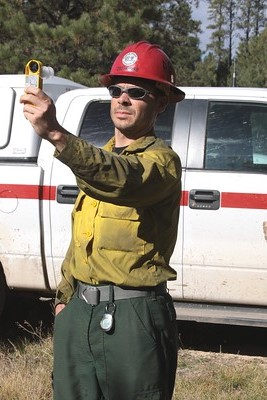
\includegraphics[width=2.2in, 
		trim={0cm 3cm 1cm 1cm}, clip=true]
		{science/weather/UsingKestrel}
		\caption{Devices like portable weather meters make it easy to quickly collect fire weather information to support tactical decisionmaking and ecological research.  
		\label{fig:UsingKestrel} } 
		% (Fig.~\ref{fig:UsingKestrel})
	\end{center}
\end{marginfigure}

Wildland fire weather information can be divided into two components \citep{teie2018}: 

 \begin{itemize}[noitemsep]
	\item \textbf{Strategic weather\textemdash}Information on general trends for a day, extending to several days. 
	\item \textbf{Tactical weather\textemdash}Local observations made at the scene (Fig.~\ref{fig:UsingKestrel}).
Typically includes air temperature (often called \emph{dry bulb}), relative humidity, and a wind vector (direction, average sustained wind speed, peak gust).
\end{itemize}

Below we describe how to acquire and use both types of data in a prescribed fire operation.
From an operational perspective, strategic weather information consists of forecasts and tactical weather information comes from belt weather kits and local automated weather stations. 
Researchers have access to the same forecast data but also historical data at multiple scales, from automatic weather stations that log data and are networked, to broad-scale, gridded historical weather data products. 

\section{Strategic weather}

Strategic weather products consist primarily of forecasts available from a number of sources at several different spatial and temporal scales.\footnote{We focus here on shorter-term products from the National Oceanic and Atmospheric Administration's National Weather Service (\href{https://www.weather.gov}{weather.gov}), but NOAA's \href{https://www.spc.noaa.gov/products/fire\_wx/overview.html}{Storm Prediction Center} and \href{https://www.cpc.ncep.noaa.gov/products/Drought/}{Climate Prediction Center} also offer longer-term outlooks relevant to fire planning.
	Additionally, the National Interagency Fire Center's Predictive Services provide a lot of fire-specific weather information at both national and regional levels (\href{https://www.predictiveservices.nifc.gov/weather/weather.htm}{predictiveservices.nifc.gov/weather/weather.htm}). 
	The information is geared towards wildland fire suppression but is also useful for prescribed fire operations. }

\subsection{Forecast products} 

The National Weather Service (NWS) provides several products either specifically for, or very relevant to, fire weather. 
We discuss a few here, starting at spatially-broad and long time scales, working to local predictions for specific time periods at a specific point on the landscape. 

\subsubsection{Basic weather products}
NWS provides extended outlooks at a national scale (Fig.~\ref{fig:ExtendedOutlookExample}). 
Each NWS office also provides a daily Area Forecast Discussion that not only explains how current regional atmospheric patterns affect the area's weather, but also some of the considerations taken into account by local forecasters as they assess model output.

\begin{figure} 
	\begin{center}
		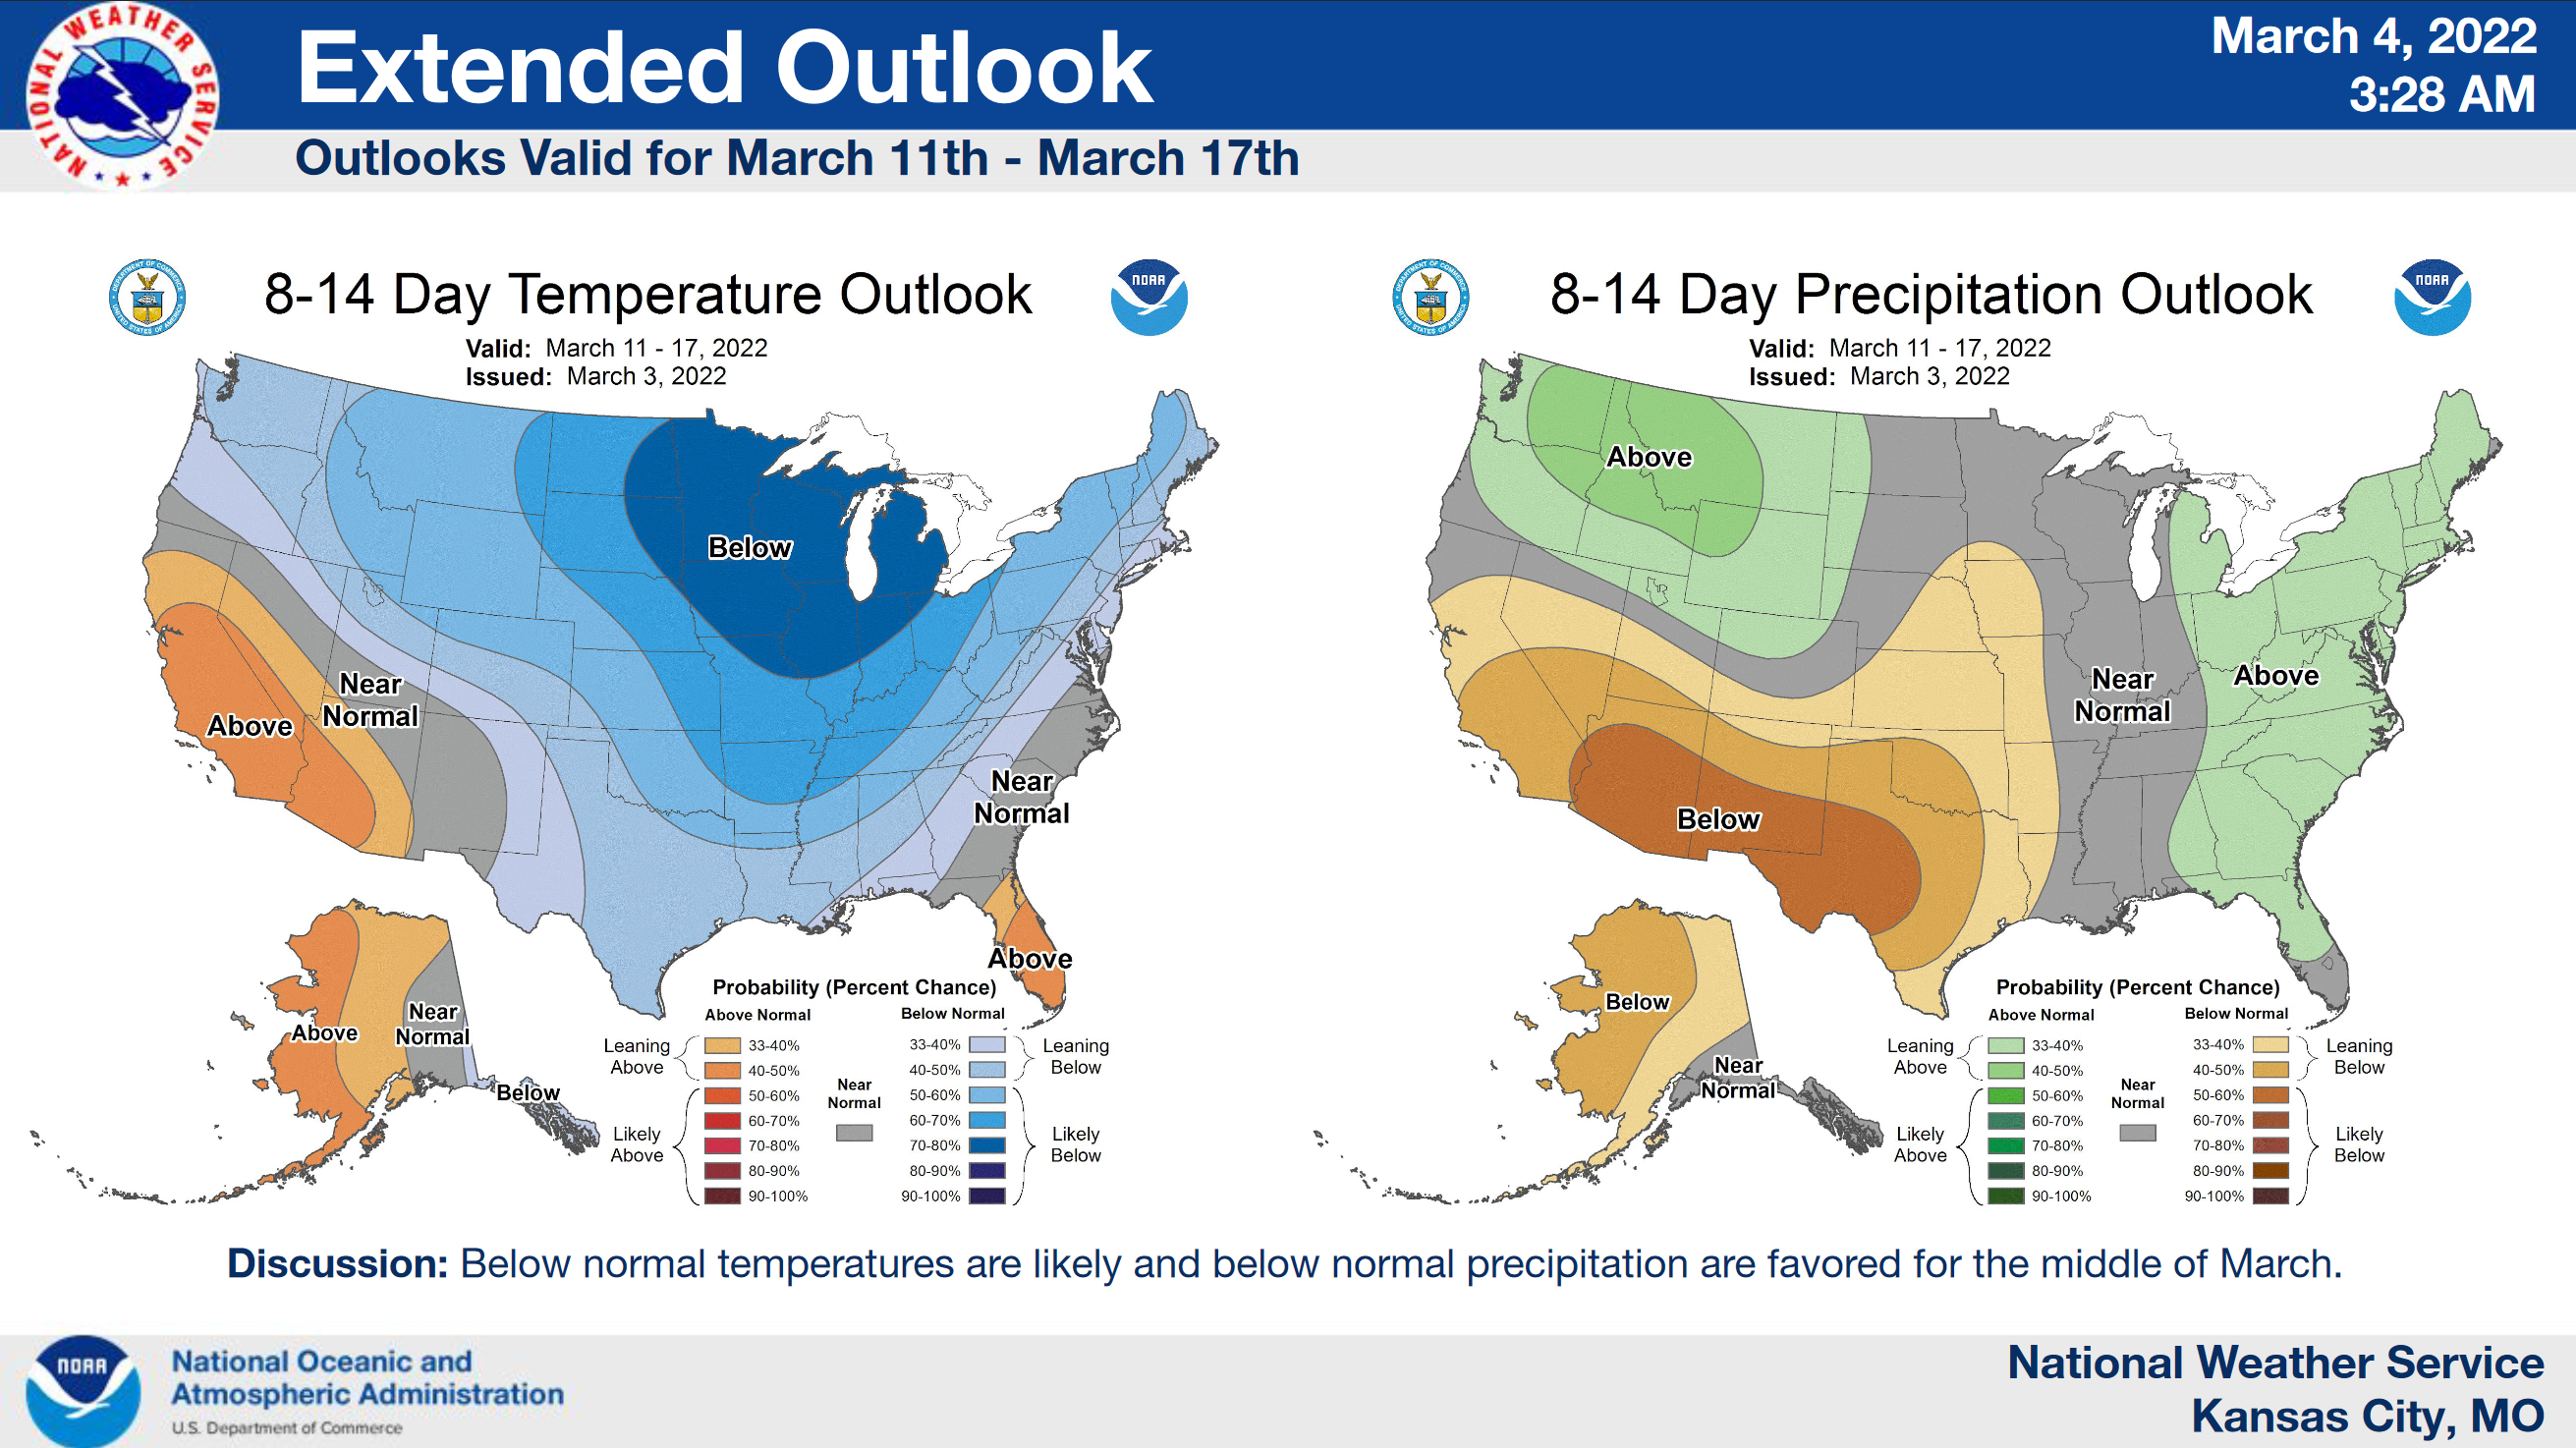
\includegraphics[width=1\textwidth]
		{science/weather/ExampleNationalExtendedOutlook}
		\ImageCredit{https://www.weather.gov/media/eax/DssPacket.pdf, 4 March 2022}
	\end{center}
	\caption{An example of national 8-14 day temperature and precipitation outlooks provided by the Kansas City, MO NWS office.
	} \label{fig:ExtendedOutlookExample}
	%(Fig.~\ref{fig:ExtendedOutlookExample})
\end{figure} 

Zone area forecasts\textemdash accessible by searching a town name at \href{http://weather.gov}{weather.gov}\textemdash are local forecasts generated at the county or municipality level by regional NWS offices.
Zone area forecasts provide a 7-day weather forecast and current conditions at the nearest NWS observation point, typically the closest airport. 
These pages also provide hourly weather forecasts that illustrate predicted trends in several weather variables hour-by-hour over the next few days (Fig.~\ref{fig:BasicHourlyExample}).

\begin{figure} 
	\begin{center}
		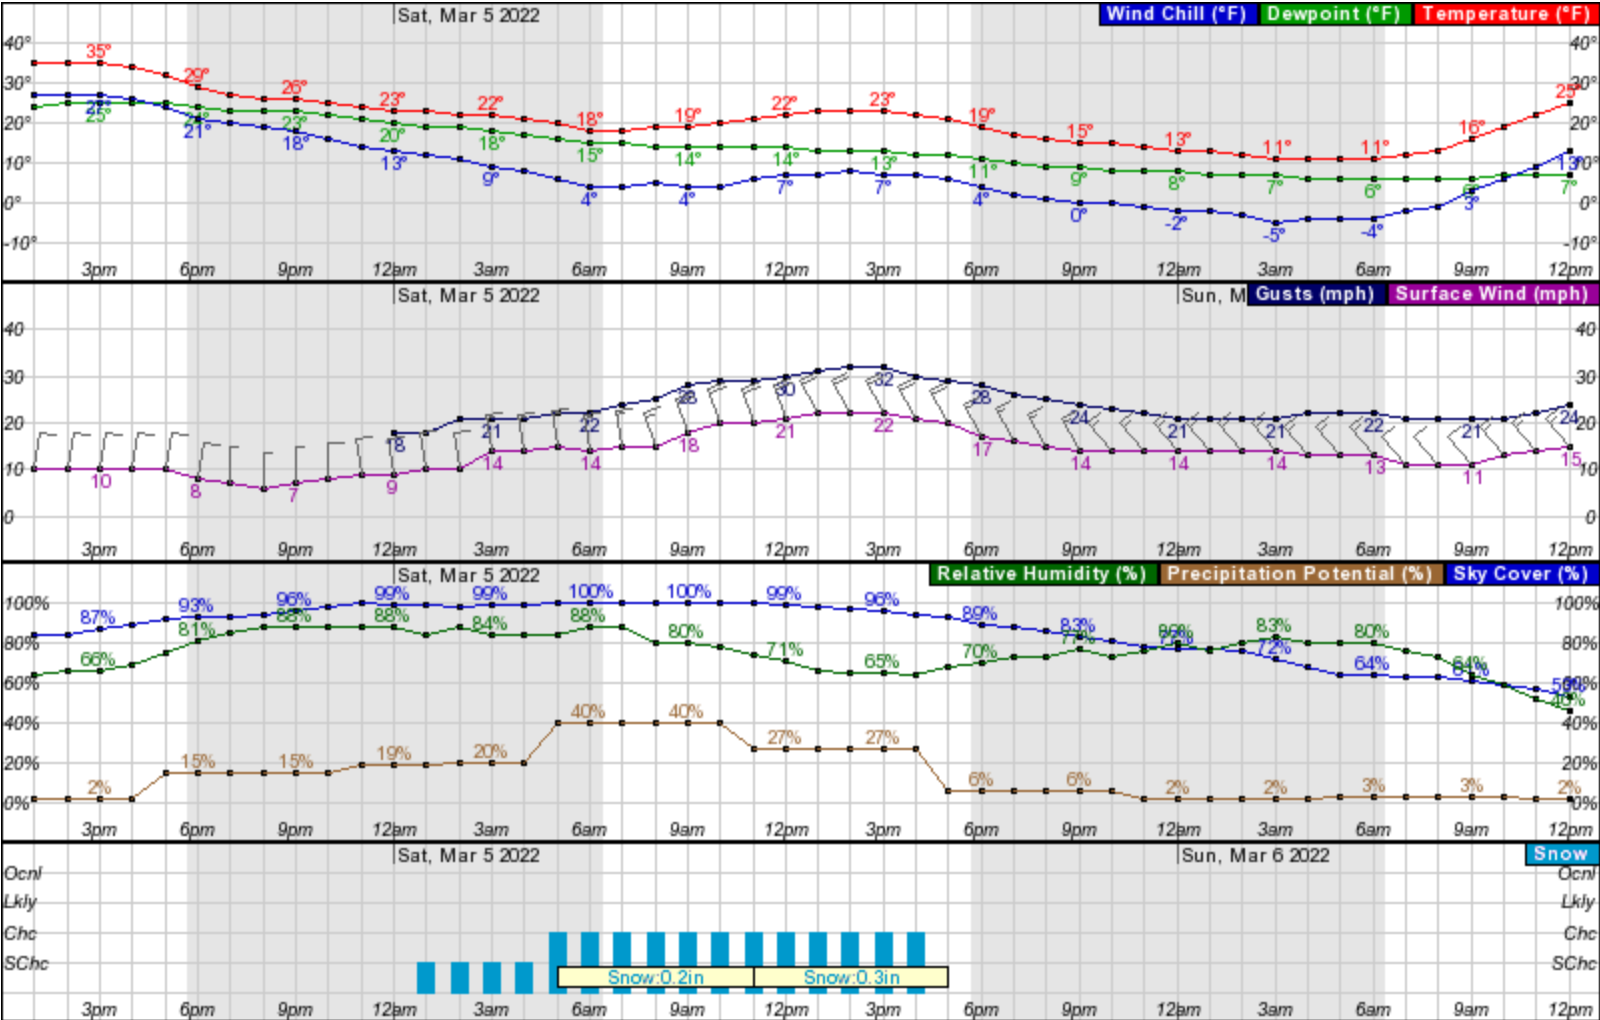
\includegraphics[width=1\textwidth]
		{science/weather/BasicHourlyExample}
	\end{center}
	\caption{An example of predicted hourly trends in several basic weather variables for two days in Hettinger, North Dakota. 
		All regional NWS offices in the country provide this product.
		While searched best by town names (\href{http://www.weather.gov}{weather.gov}), one can edit the latitude and longitude fields in the URL by hand to generate an hourly forecast for a specific point and bookmark it for future use. 
	} \label{fig:BasicHourlyExample}
	%(Fig.~\ref{fig:BasicHourlyExample})
\end{figure}  

\subsubsection{Specific fire weather products} 

\begin{figure}
	\caption{Two examples of national fire-related forecast products conveniently posted at \href{https://www.weather.gov/fire/}{weather.gov/fire}, but produced elsewhere: the wildfire potential outlook product is generated by the \href{https://www.predictiveservices.nifc.gov}{National Interagency Fire Center's Predictive Services} while the drought monitor comes from the \href{https://droughtmonitor.unl.edu/}{University of Nebraska\textendash Lincoln}. 
	} 
	\begin{center}
		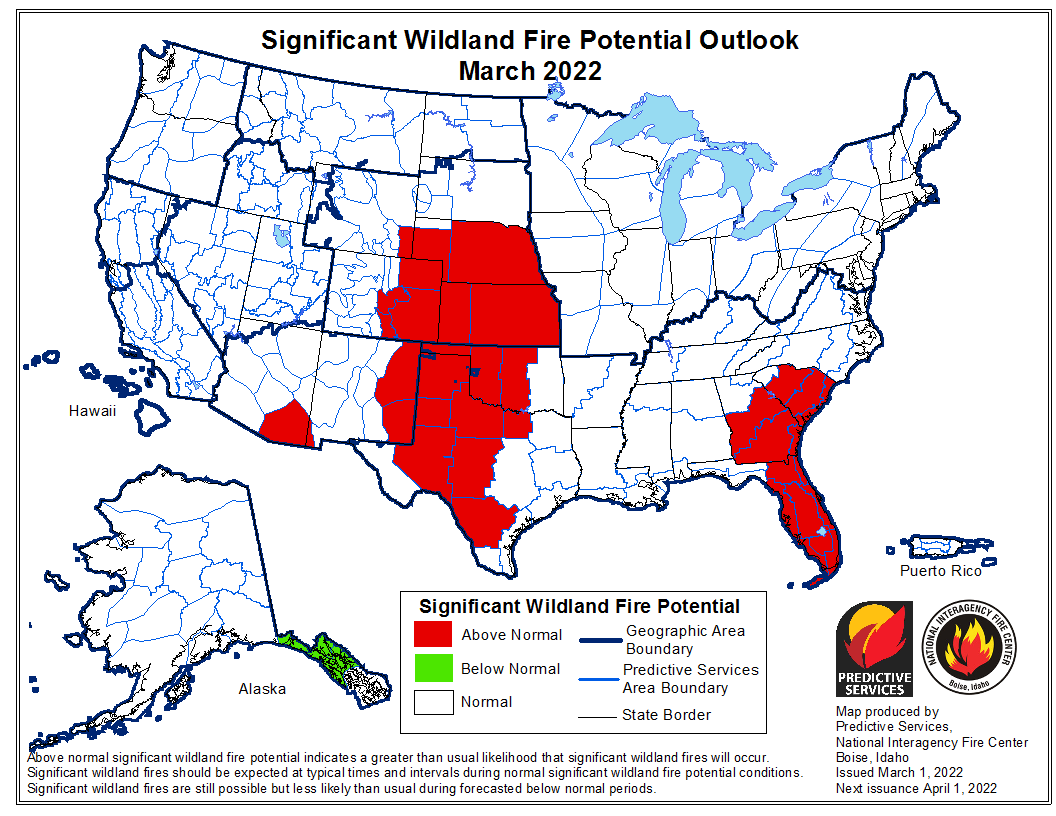
\includegraphics[width=0.5\textwidth]
		{science/weather/MonthOutlookExample}~
		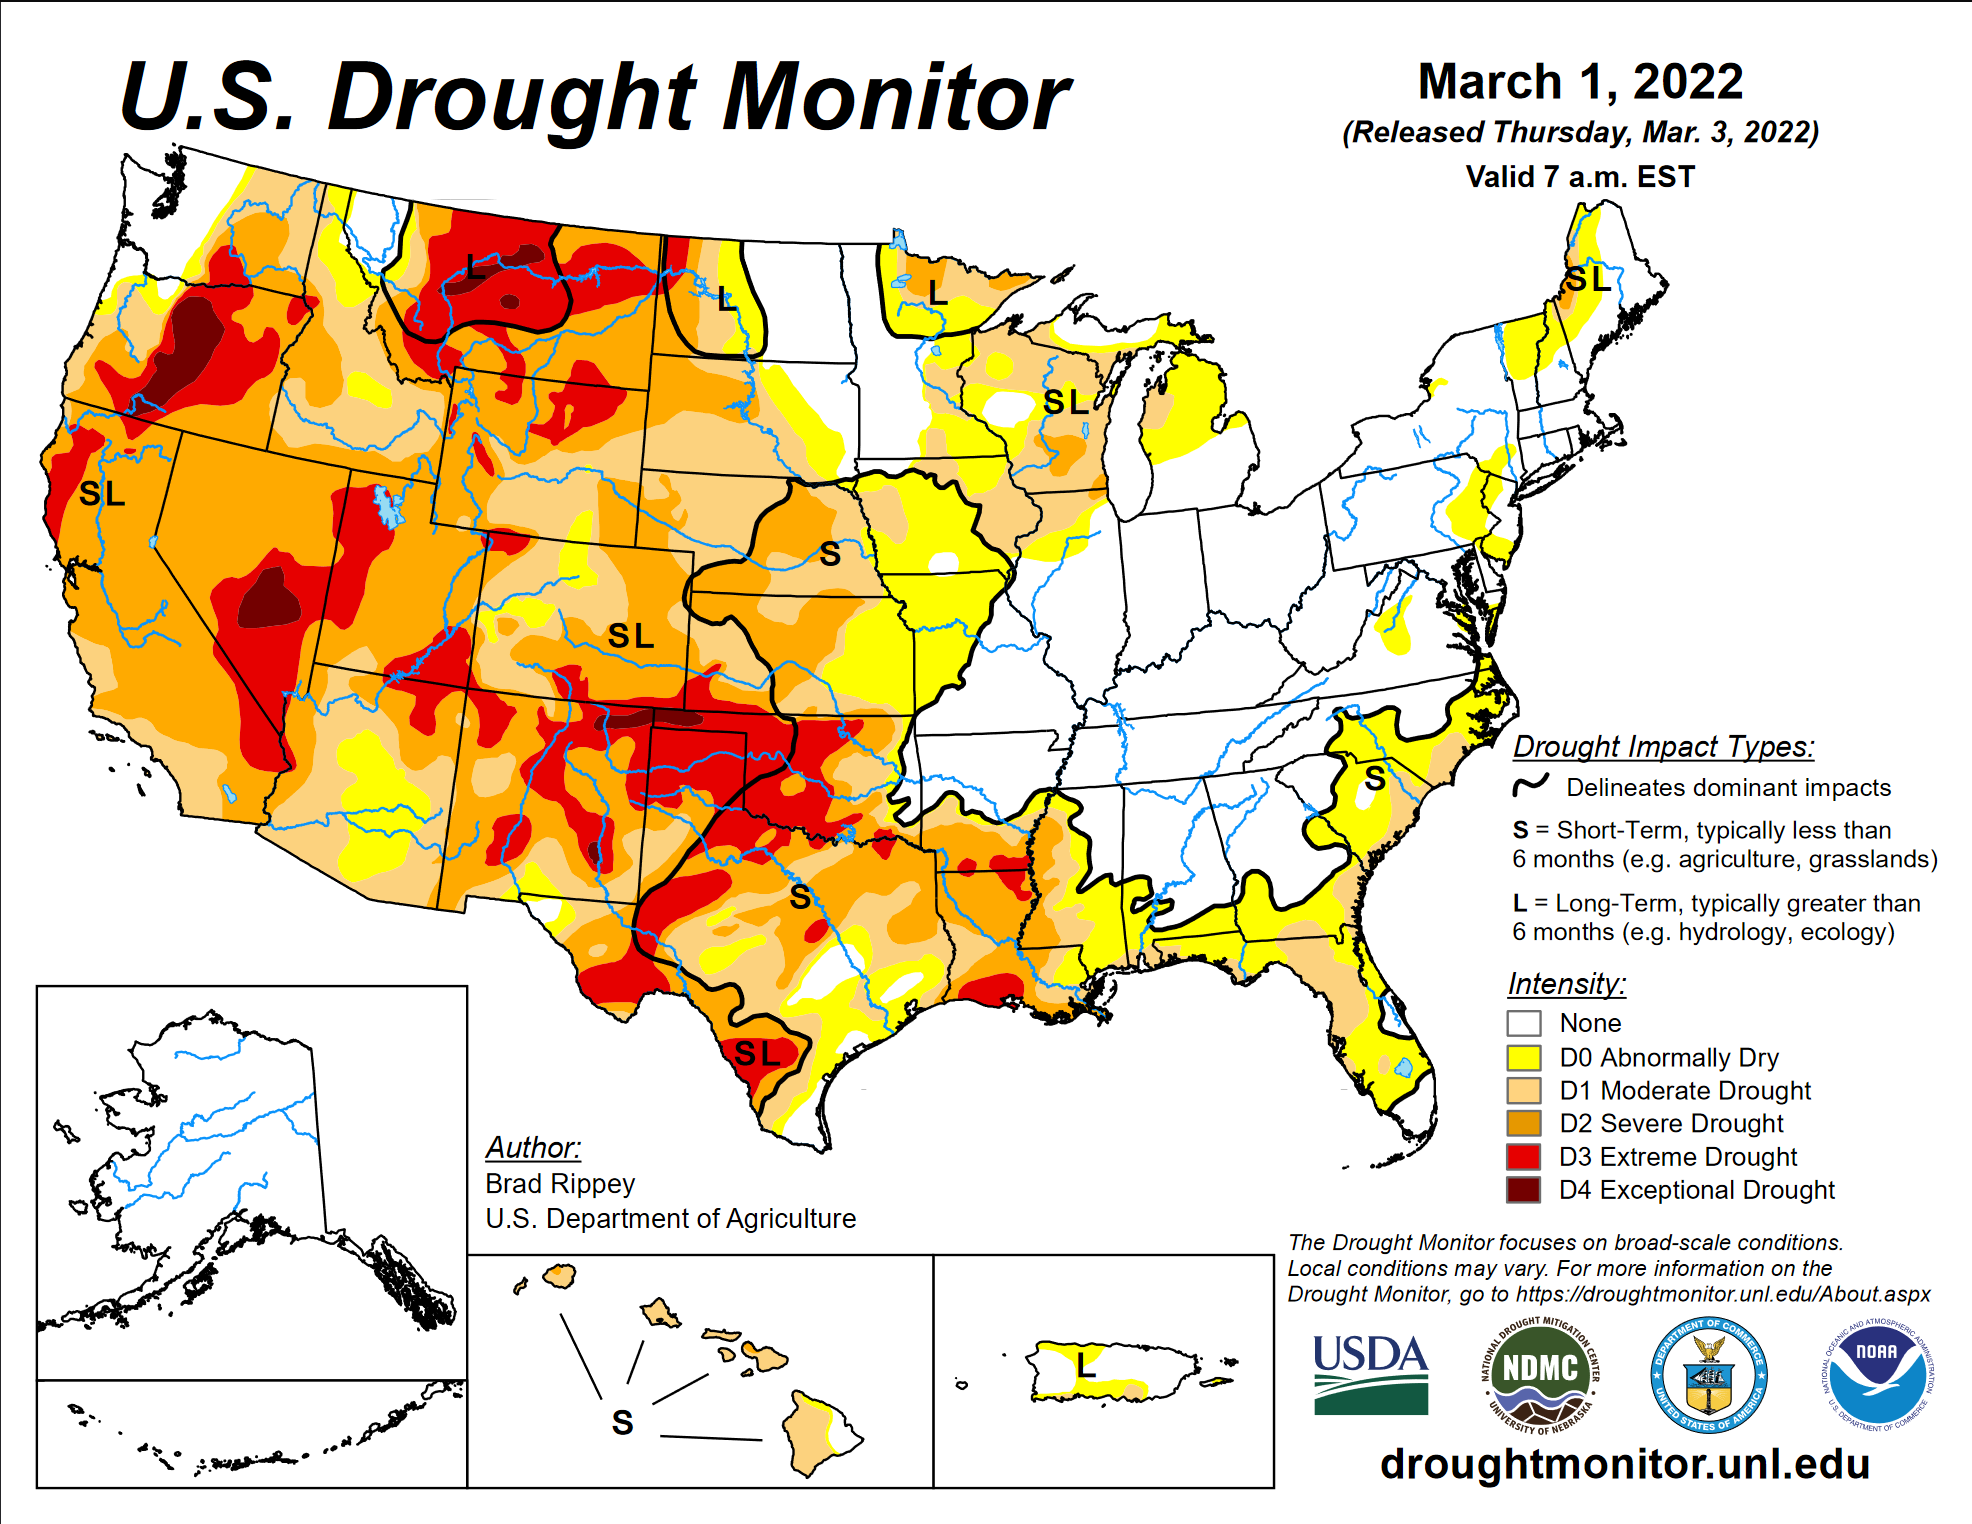
\includegraphics[width=0.5\textwidth]
		{science/weather/DroughtMonitorExample}
	\end{center}
	\label{fig:NationalProducts}
	%(Fig.~\ref{NationalProducts})
\end{figure}

National fire-related forecast data are compiled at \href{https://www.weather.gov/fire/}{weather.gov/fire (Fig.~\ref{NationalProducts})}. 
Some regional NWS offices provide fire-specific forecast information. 
\href{https://forecast.weather.gov/product\_sites.php?site=NWS\&product=FWF}{Several regional offices around the country} provide text-based Routine Fire Weather Forecasts that give strategic fire weather forecasts for smaller zones within the area (Fig.~\ref{fig:RoutineFireFcstExample}).
But not all offices provide fire-specific data, and not all regions provide the same information or even for the whole year.
For example, Bismarck, ND regional office has \href{https://www.weather.gov/bis/fire\_managers}{a page dedicated to fire weather in western and central North Dakota}, but it isn't maintained during winter months.
And compare differences in output between Figs.~\ref{fig:RoutineFireFcstExample} \& \ref{fig:SpotExample} due to different local environmental contexts.  

\begin{figure} 
	\begin{center}
		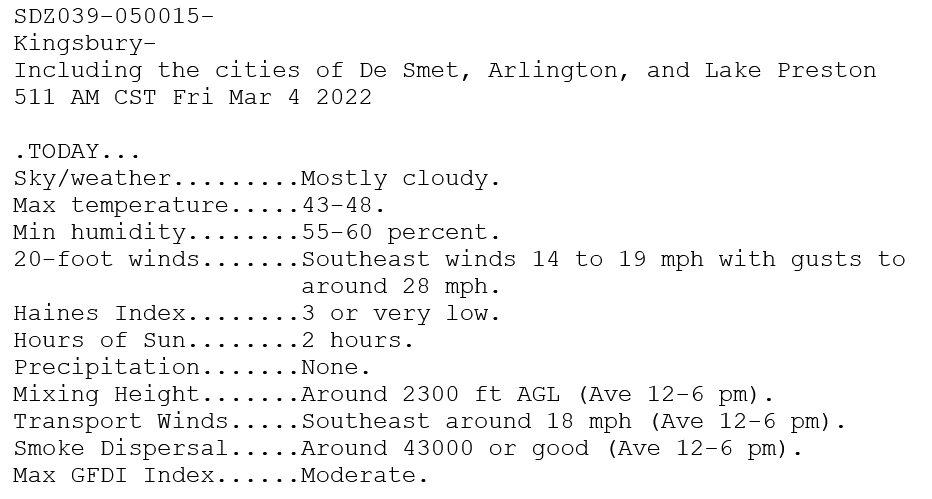
\includegraphics[width=1\textwidth]
		{science/weather/RoutineFireFcstExample}
	\end{center}
	\caption{An example of a Routine Fire Weather Forecast for Kingsbury County, South Dakota. 
		Note that because much of South Dakota wildland fire occurs in rangeland, many NWS offices in the state calculate a Grassland Fire Danger Index (GFDI). 
	} \label{fig:RoutineFireFcstExample}
	%(Fig.~\ref{fig:RoutineFireFcstExample})
\end{figure}  

\paragraph{Spot weather forecasts}
	
A spot weather forecast is a ''special forecast issued to fit the time, topography, and weather of a specific incident.''\footnote{\citet[Spot Weather Forecast][]{nwcg2019}}
The forecast includes information similar to the routine fire weather forecast  (Fig.~\ref{fig:RoutineFireFcstExample}), but a specific NWS forecaster concentrates predictive weather models on a specific location provided by a request filed by a qualified user at \href{https://www.weather.gov/spot/}{weather.gov/spot}. 
Requests include the geospatial location and date along with some site-specific information, such elevation above sea level, fuel type, slope and aspect, and size of burn. 
The results include a description of general weather patterns expected for the day, as well as specific predicted values for fire-related variables at critical points in the day (Fig.~\ref{fig:SpotExample}).

\begin{figure} 
	\begin{center}
		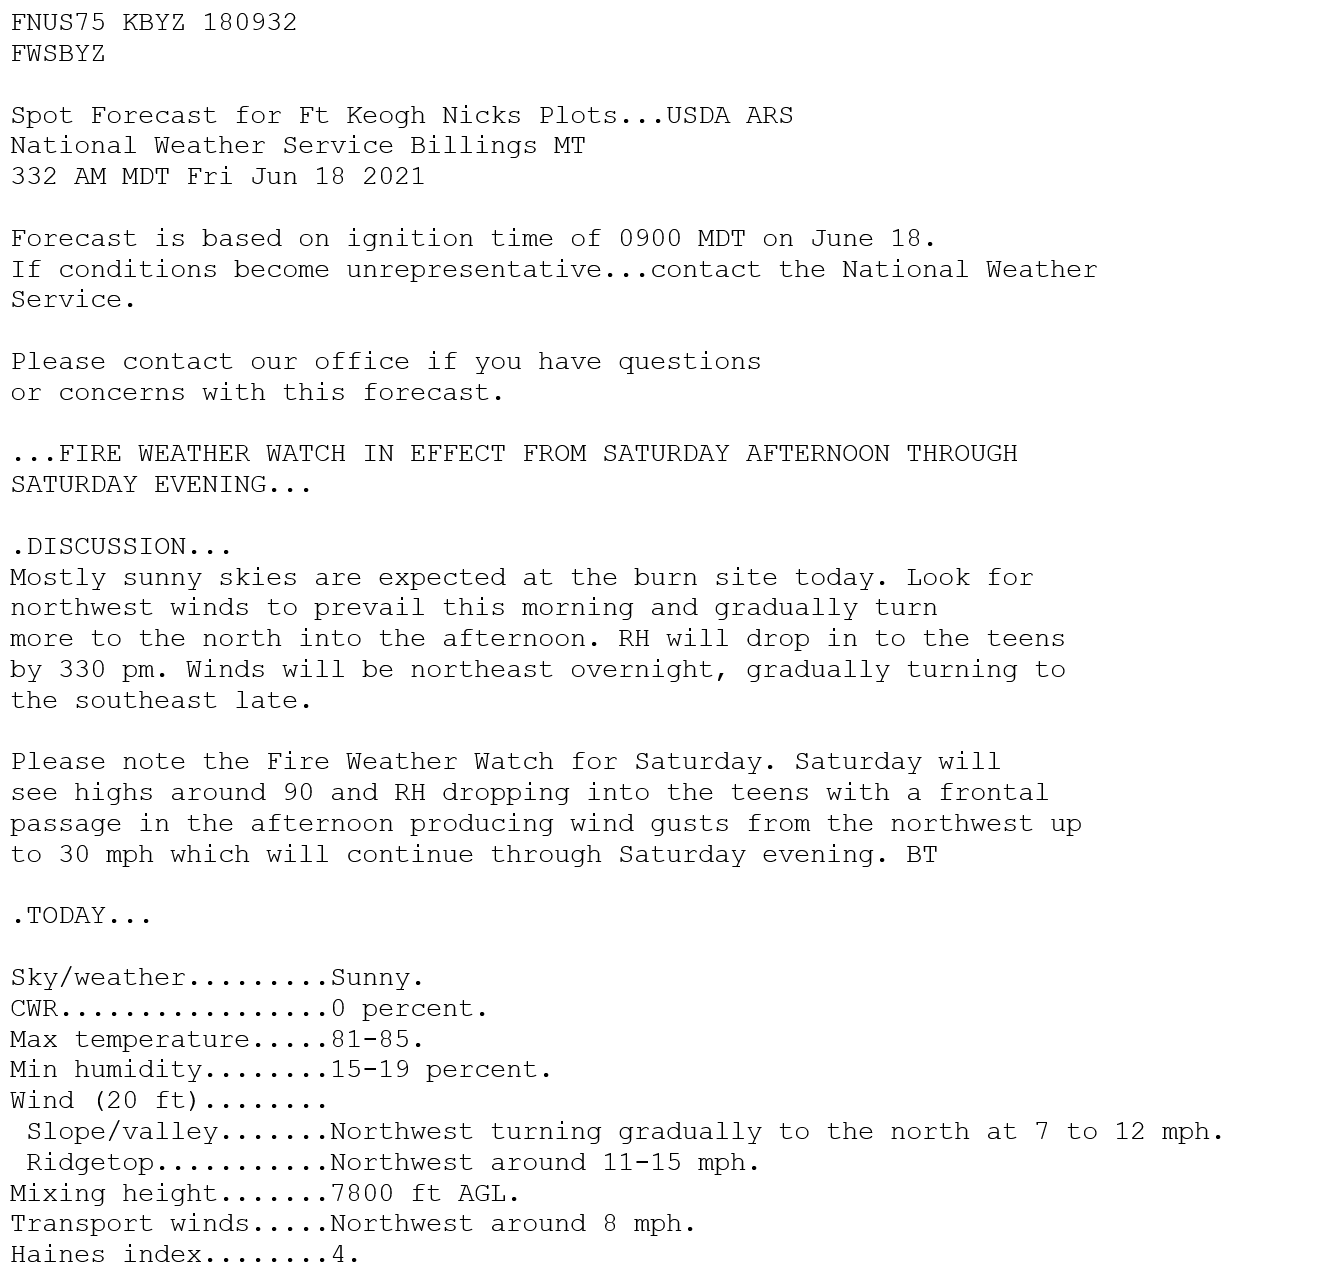
\includegraphics[width=1\textwidth]
		{science/weather/SpotExample}
	\end{center}
	\caption{An example of a Spot Weather Forecast for a summer prescribed burn generated by the NWS regional office in Billings, MT.
		Note that because the Billings office covers mountainous areas, forecasters account for topographical effects on wind by breaking wind predictions  down for slope/valley and ridgetop positions. 
		Note also that the forecast was generated at 03:33, and the forecaster calls attention to a fire weather watch in effect for the next day, with a description of the anticipated weather changes. 
		As the ignition time approached and observed winds were higher than predicted, the NWS staff member who generated the spot forecast contacted the burn boss via the cell phone number provided in the request. 
		After a discussion with local fire management officials about existing fire danger conditions and the expected trend towards extreme weather, this prescribed fire operation was postponed. 
		It is impossible to determine whether this burn would have been a success or a failure had the burn boss proceeded. 
		But by working with the NWS and county officials, the burn boss was certainly aware of the current and forecast conditions when considering the Go/No-go decision. 
	} \label{fig:SpotExample}
	%(Fig.~\ref{fig:SpotExample})
\end{figure} 

The official NWS spot forecast process is not the only way to obtain location-specific information. 
Regional offices that provide fire services also provide fire-specific products in the hourly weather forecast format (Fig.~\ref{fig:FireHourlyExample}). 
Even managers who obtain official spot weather forecasts can complement that information, which focuses on weather at critical times of the day, with hourly predictions of the same fire-specific variables. 

\begin{figure} 
	\begin{center}
		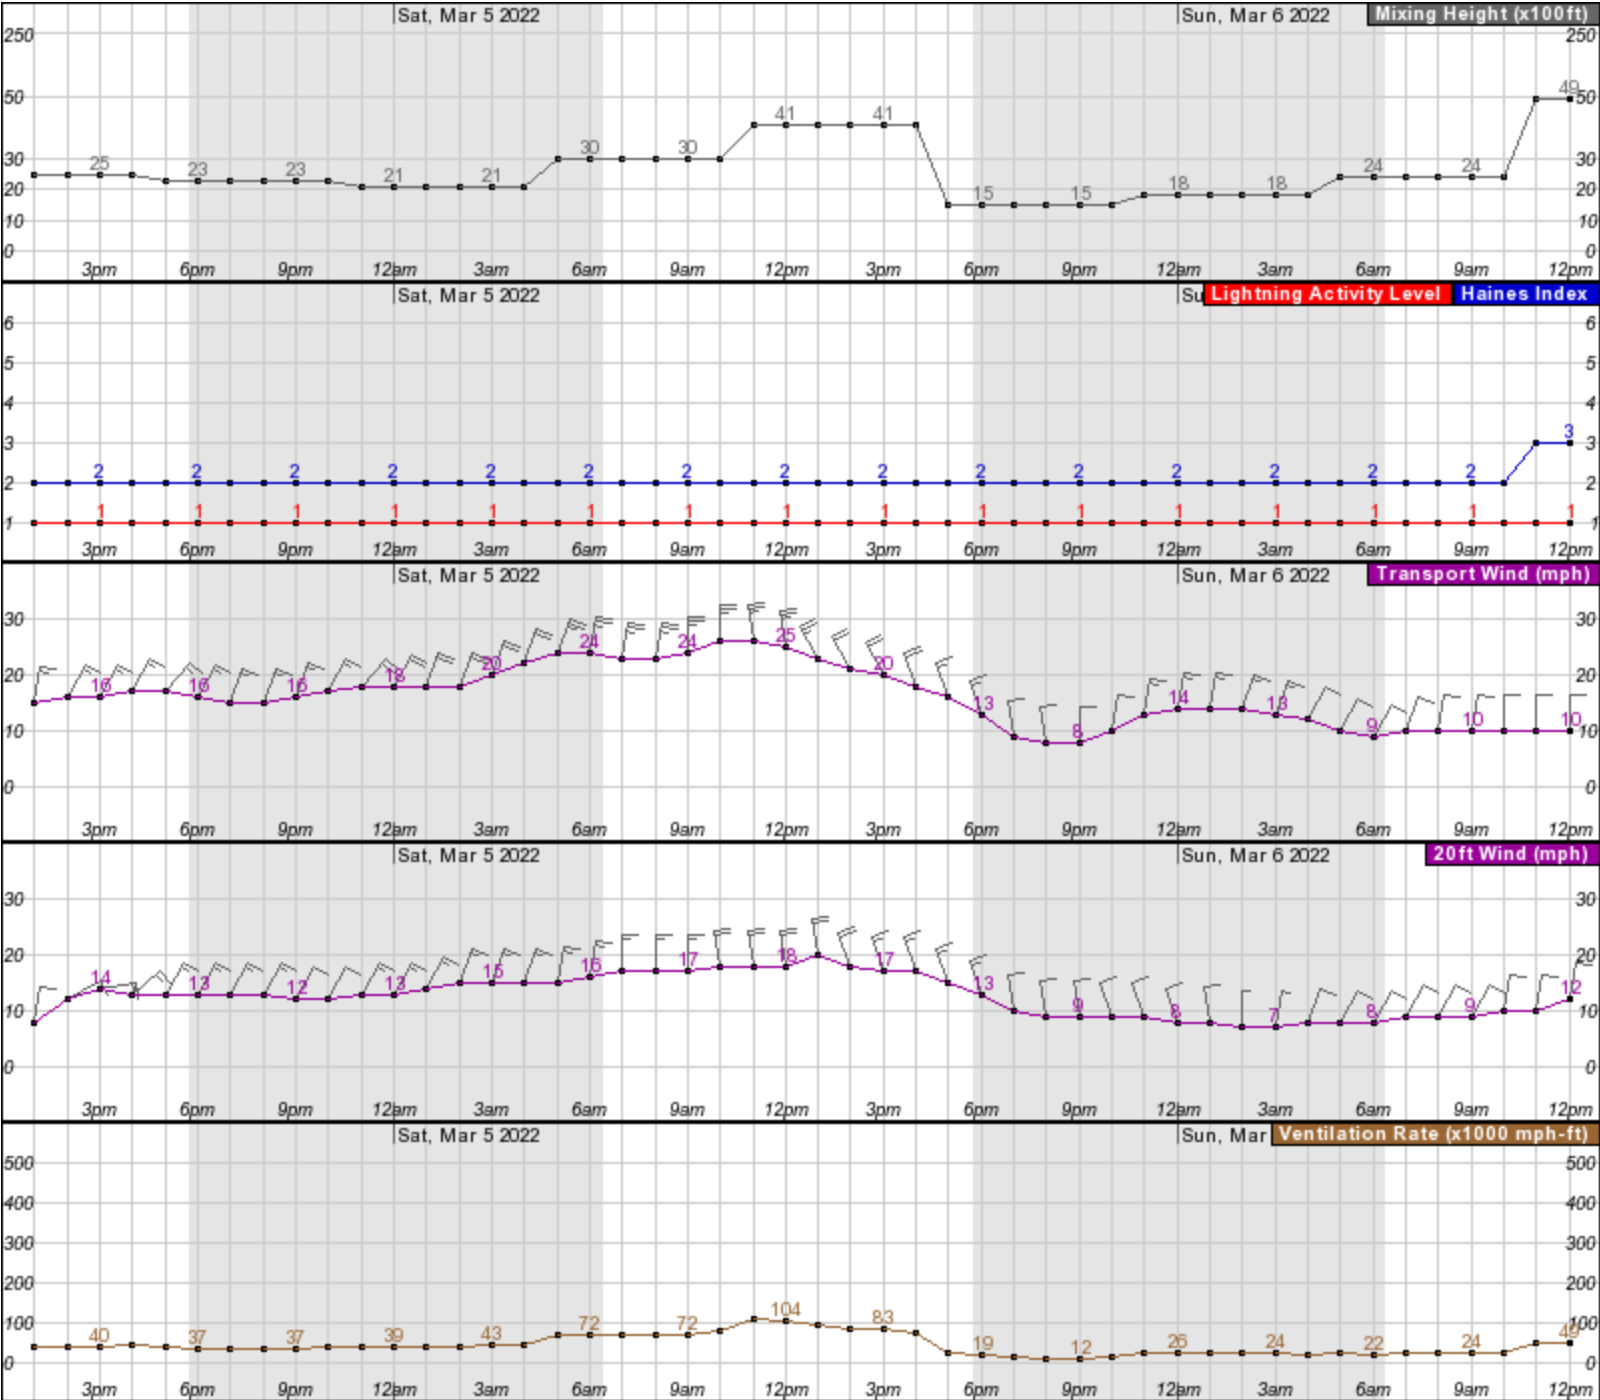
\includegraphics[width=1\textwidth]
		{science/weather/FireHourlyExample}
	\end{center}
	\caption{An example of predicted hourly trends in several variables specific to wildland fire for two days in Chadron, Nebraska. 
		Not all regional NWS offices in the country provide fire products, and the specific fire products provided varies among offices. 
		The hourly weather format can be ``hacked'' to provide location-specific information by hand-editing the longitude and latitude fields of the URL for an hourly weather product found for a local town.
	} \label{fig:FireHourlyExample}
	%(Fig.~\ref{fig:FireHourlyExample})
\end{figure}  

\section{Tactical weather}

Fire managers and researchers alike rely on real-time fire weather observations taken during the operational period.

\begin{figure} 
	\begin{center}
		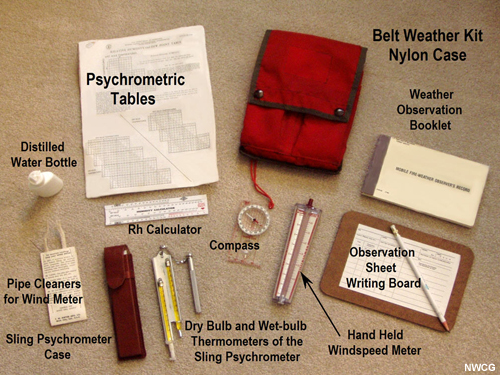
\includegraphics[width=1\textwidth]
		{science/weather/BeltWeatherKit}
	%	\ImageCredit{NWCG}
	\end{center}
	\caption{Standard items in the belt weather kit for making fire weather observations in the field. 
	} \label{fig:BeltWeatherKit}
	%(Fig.~\ref{fig:BeltWeatherKit})
\end{figure} 

\subsection{Spinning weather}

The tried-and-true methods of taking fire weather measurements are included in the \emph{belt weather kit}, a standard package of field-ready instruments for measuring and recording air temperature, dew point \& relative humidity, and wind speed \& direction (Fig.~\ref{fig:BeltWeatherKit}). 
Using the belt weather kit is sometimes called \emph{spinning weather} in reference to the sling psychrometer that is used for measuring dew point and relative humidity. 

While the belt weather kit has been technologically superceded by portable handheld weather meters (Fig.~\ref{fig:UsingKestrel}), it remains important to understand the operation of the belt weather kit because both methods have their own sources of error and opportunities for malfunction or damage. 
And one never knows when the batteries on the electronic meter will fail.
Finally, there is debate on which method is ``best.'' 
When both options are available, fire weather observers are advised to use both the belt weather kit and an electronic meter at least at the beginning of the observation period and make a note of which method was used to collect each value.  

Common tactical weather variables include: 

\begin{itemize}%[noitemsep]
	\item \textbf{Air temperature\textemdash}Often called \emph{dry bulb temperature} because ambient air temperature can be read from the unaltered thermometer on the sling psychrometer. 
	Air temperature is not a direct factor in fire behavior, but it helps managers understand trends in fuel moisture and crew well-being. 
	\item \textbf{Relative humidity (RH)\textemdash}As a measure of the capacity for the air to absorb moisture, RH is a critical variable in how quickly fuel dehydrates, and thus fire intensity. 
	Exposure to low RH desiccates fuels ahead of flame fronts and makes crew members more susceptible to dehydration. 
	RH is calculated by comparing measurements from a sling psychrometer via a psychrometic table or slide rule (Fig.~\ref{fig:SpinningWeather}, \emph{top}). 
	\item \textbf{Wind\textemdash}Wind is often reported as a \emph{vector} consisting of velocity and speed. 
	As ventilation increases oxygen available to the combustion reaction zone, wind increases fire intensity and drives rate of spread.  
	Wind speed is often reported as \emph{sustained}\textemdash an average value or range of wind speed over a minute or two\textemdash and \emph{gusts}\textemdash peak velocities that are substantially above the average or beyond the range of sustained winds. 
	Handheld anemometers measure wind speed (Fig.~\ref{fig:SpinningWeather}, \emph{bottom}). 
	A compass aids in determining wind direction. 
\end{itemize}

\begin{figure} 
	\begin{center}
		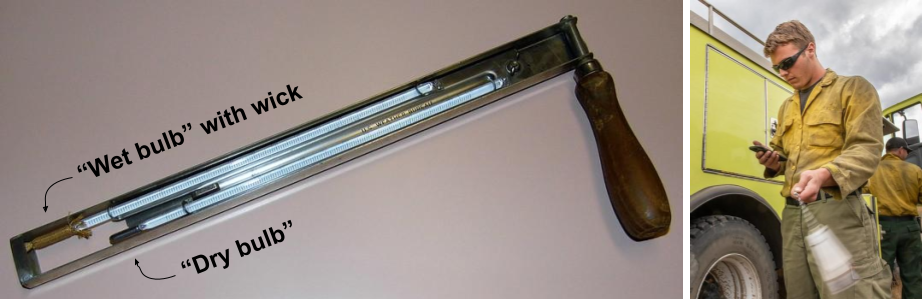
\includegraphics[width=1\textwidth]
		{science/weather/SlingPsychrometer}\\
		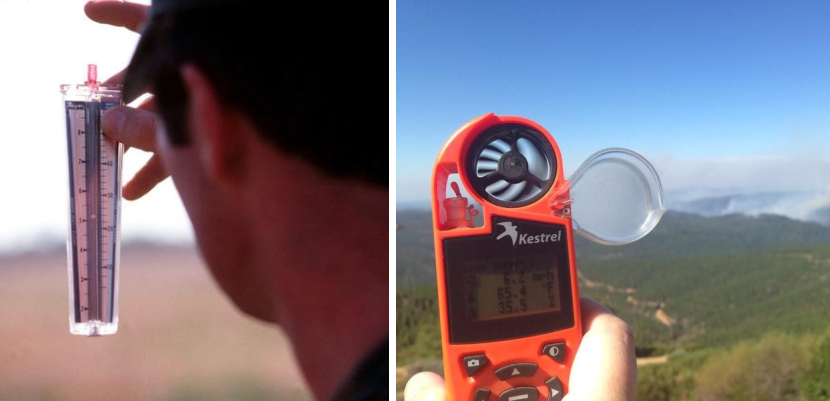
\includegraphics[width=1\textwidth]
		{science/weather/anemometers}
		\ImageCredit{TL: Joe Haupt, CC BY-SA 2.0; TR: Neal Herbert, US DOI, public domain; BL: USAF, public domain; BR: USDA, CC BY 2.0}
		\ImageIndex{CC BY-SA 2.0}
		{fig:SlingPsychrometer}
		{Joe Haupt}
		{https://www.flickr.com/photos/51764518@N02/19543105108}
	\end{center}
	\caption{Methods of taking fire weather observations. 
		\textbf{Top:} Sling psychrometers allow one to calculate instantaneous relative humidity by determining how quickly evaporation produces a cooling effect. 
		Left: An antique sling psychrometer with a wooden handle for spinning two thermometers, one open to the ambient air (``dry bulb'') and one with a ``wet bulb'' wrapped in a soaked wick that cools while the water evaporates while the device is spun rapidly. 
		A table or slide rule in the belt weather kit converts the difference between the final temperatures into dew point (DP) and relative humidity (RH). 
		Right: Belt weather kits include a small sling psychrometer with a chain connecting the thermometers to a chain, and smartphone apps quickly calculate DP and RH. 
		\textbf{Bottom:} Two methods for determining wind speed. 
		Left: Analog wind meter, standard in the belt weather kit. 
		Right: A Kestrel brand all-in-one portable weather kit. 
		Such units take digital measurements of many parameters of use to wildland fire professionals. 
	} \label{fig:SpinningWeather}
	%(Fig.~\ref{fig:SpinningWeather})
\end{figure}



\subsection{Automated weather stations} 

Additionally, hourly weather observations made by the NWS and even Remote Access Weather Stations managed by state and federal agencies are all available together online at MesoWest \href{https://mesowest.utah.edu/}{mesowest.utah.edu}. 


\section{Historical weather data}



\paragraph{Point-level data} 

Many of the same resources for getting real-time observations from remote weather stations provide a means to access historical records. 
Substantial requests for historical MesoWest data can be managed via their ``official'' API service \href{https://developers.synopticdata.com/mesonet/}{https://developers.synopticdata.com/mesonet/}, the \href{https://github.com/fickse/mesowest}{\emph{mesowest}} R package, and the \href{https://github.com/mesowx/MesoPy}{\emph{MesoPy}} python package.

\paragraph{Local data}

One of the best resources for historical weather in the US is gridMET \citep{abatzoglou2013}, ``a dataset of daily high-spatial resolution (\~4-km, 1/24th degree) surface meteorological data covering the contiguous US from 1979-yesterday. (\href{https://www.climatologylab.org/gridmet.html}{climatologylab.org/gridmet.html})''
Values represent data extremes (maximum temperature, minimum RH) interpolated for grid cells across the US via models using data from several weather observation networks. 
The gridMET dataset includes several fire weather variables (e.g., dry bulb temperature, relative humidity, dew point, and wind vectors) as well as indicators of potential fire behavior including products from the National Fire Danger Rating System (100-hr fuel moisture, Burning Index \& Energy Release Component). 
In addition to the steps listed on their website, gridMET data can be accessed via the \href{https://github.com/mikejohnson51/climateR/}{\texttt{climateR}} R package  and \href{https://explorer.earthengine.google.com/#detail/IDAHO\_EPSCOR\%2FGRIDMET}{Google Earth Engine}. 

 \begin{marginfigure}
	\begin{center}
		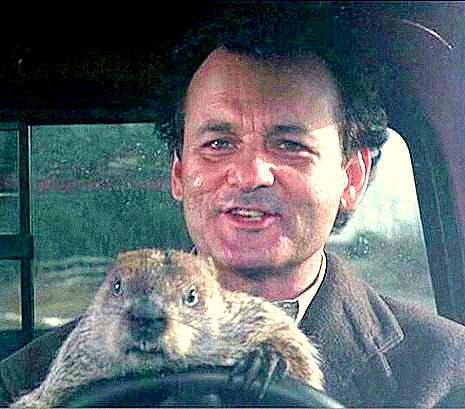
\includegraphics[width=2.2in, 
		trim={1.5cm 0cm 1cm 0.5cm}, clip=true]
		{groundhogday}
		\caption{Topography, weather, and the fuelbed are the three major drivers of wildland fire behaviour.
			\index{Fire triangles!Fire behaviour|textit} \label{fig:groundhog} } 
		% (Fig.~\ref{fig:groundhog})
	\end{center}
\end{marginfigure}